\documentclass[a4paper,twoside]{memoir}
% Set up encoding

\usepackage{graphicx,color}
\definecolor{black}{rgb}{0,0,0}
\makeatletter
\newlength{\numberheight}
\makechapterstyle{TroelsPedersen}{%
\setlength{\beforechapskip}{-20pt}
\setlength{\midchapskip}{0pt}
\setlength{\afterchapskip}{40pt}
\renewcommand{\chapnamefont}{\normalfont\LARGE\itshape}
\renewcommand{\chapnumfont}{\normalfont\HUGE\itshape\color{black}}
\renewcommand{\chaptitlefont}{\normalfont\HUGE\itshape\color{black}}
\renewcommand{\afterchapternum}{}
\renewcommand{\printchaptername}{}
\setlength{\numberheight}{20mm}
\renewcommand{\chapternamenum}{}%
\renewcommand{\printchapternum}{%
\sidebar{\makebox[0pt][l]{%
\resizebox{!}{\numberheight}{\chapnumfont\thechapter}}}}%
\renewcommand\printchaptertitle[1]{\chaptitlefont##1}
}
\makeatother
\chapterstyle{TroelsPedersen}

\usepackage[utf8]{inputenc}

% Mulighed for at definere acronyms
\usepackage{acronym}

%package for linenumbers
\usepackage{lineno} 

% Load up bibliography.
\usepackage[authoryear]{natbib}
\setcitestyle{numbers,square}
% Bibliography style.
\bibliographystyle{plainnat}

% Algorithm support.
\usepackage{algorithmic}
\usepackage{algorithm}
\usepackage{subfig}
\usepackage{amsmath}
\usepackage{amsfonts}
% Make algorithms appear as procedures instead.
\floatname{algorithm}{Procedure}
\renewcommand{\algorithmicrequire}{\textbf{Input:}}
\renewcommand{\algorithmicensure}{\textbf{Output:}}

% Image frames.
\setlength{\fboxsep}{0pt}
\setlength{\fboxrule}{0.5pt}

% Also, images.
\usepackage{graphicx}

% tabeller der strækker sig over flere sider
\usepackage{longtable}

% flere tabel-muligheder
\usepackage{multirow}

% bedre enumerate
\usepackage{enumitem}

% Mulighed for if-then-else sætning!
\usepackage{ifthen}

% Todo notes here and there.
% write instead for disable: \usepackage[disable]{todonotes}
\usepackage{todonotes}

% Forbedrede floats.
\usepackage{float}
\usepackage{rotating}

\newsubfloat{figure}

% Special symbols availability.
\usepackage{amssymb}

% Email @
\usepackage{marvosym}

%Degree symbol
\usepackage{gensymb}

% Wrap figure
\usepackage{wrapfig}

% Remove subsection numbering
\renewcommand{\thesubsection}{}
\makeatletter
\def\@seccntformat#1{\csname #1ignore\expandafter\endcsname\csname the#1\endcsname\quad}
\let\subsectionignore\@gobbletwo
\let\latex@numberline\numberline
\def\numberline#1{\if\relax#1\relax\else\latex@numberline{#1}\fi}
\makeatother

%landscape mode
\usepackage{lscape}

\usepackage{booktabs}
\usepackage{hvfloat}
\usepackage{units}

%Fun with captions
\usepackage{caption}


% Neat-o referencer...o.
\usepackage{bookmark,hyperref}
\usepackage{nameref}

\newcommand{\secref}[1]{Section \ref{#1}}
\newcommand{\chapref}[1]{Chapter \ref{#1}}
\newcommand{\appref}[1]{Appendix \ref{#1}}

% Skriver Appendix foran Appendices
\renewcommand*{\cftpartname}{PART~}
%\renewcommand*{\cftchaptername}{\chaptername~}
\renewcommand*{\cftappendixname}{\appendixname~}
%\renewcommand*{\cftchapteraftersnum}{.}% dot after the number
%\setlength{\cftchapternumwidth}{2em}

% Operationel semantik
\newcommand{\lag}{\langle}
\newcommand{\rag}{\rangle}
\newcommand{\setof}[2]{\ensuremath{\{ #1 \mid #2 \}}}
\newcommand{\set}[1]{\ensuremath{\{ #1 \}}}
\newcommand{\besk}[1]{\ensuremath{\lag #1 \rag}}
\newcommand{\ra}{\rightarrow}
\newcommand{\lra}{\longrightarrow}
\newcommand{\Ra}{\Rightarrow}

% CODE %
\usepackage{listings}
\usepackage{color}
%\usepackage{bera}
\definecolor{gray}{rgb}{0.4,0.4,0.4}
\definecolor{darkblue}{rgb}{0.0,0.0,0.6}
\definecolor{cyan}{rgb}{0.0,0.6,0.6}
\definecolor{dkgreen}{rgb}{0,.6,0}
\definecolor{dkblue}{rgb}{0,0,.6}
\definecolor{dkyellow}{cmyk}{0,0,.8,.3}

\lstset{
  basicstyle=\ttfamily,
  columns=fullflexible,
  showstringspaces=false,
  commentstyle=\color{gray}\upshape,
  basicstyle=\small,
  numberstyle=\footnotesize,
  numbers=left,
  captionpos=b,
  stepnumber=1,
  numbersep=10pt,
  tabsize=4,
  breaklines=true,
  literate=
  {æ}{{\ae}}1
  {Æ}{{\AE}}1
  {ø}{{\o}}1
  {Ø}{{\O}}1
  {å}{{\r{a}}}1
  {Å}{{\r{A}}}1
  {§}{{\S}}1
  {é}{{\'{e}}}1
}
% Define markup of XML
\lstdefinelanguage{XML}
{
  morestring=[b]",
  morestring=[s]{>}{<},
  morecomment=[s]{<?}{?>},
  identifierstyle=\color{darkblue},
  keywordstyle=\color{cyan},
  morekeywords={id, target, type, category, value, point, correct, rows, width, time}% list your attributes here
}
% Define markup of C#
\lstdefinelanguage{CSharp}[Visual]{C++}
{
	identifierstyle=\color{darkblue},
	commentstyle=\color{green!70!black}\itshape ,
	stringstyle=\color{gray},
	sensitive=true,
	morestring=[b]",
	morestring=[b]',
	morecomment=[l]//,
	morecomment=[n]{/*}{*/}
}

% Define markup of Javascript
\lstdefinelanguage{JavaScript}{
  keywords={typeof, new, true, false, catch, function, return, null, catch, switch, var, if, in, while, do, else, case, break},
  keywordstyle=\color{blue}\bfseries,
  ndkeywords={class, export, boolean, throw, implements, import, this},
  ndkeywordstyle=\color{darkgray}\bfseries,
  identifierstyle=\color{black},
  sensitive=false,
  comment=[l]{//},
  morecomment=[s]{/*}{*/},
  commentstyle=\color{purple}\ttfamily,
  stringstyle=\color{red}\ttfamily,
  morestring=[b]',
  morestring=[b]"
}

% Define markup of Java
\definecolor{dkgreen}{rgb}{0,0.6,0}
\definecolor{gray}{rgb}{0.5,0.5,0.5}
\definecolor{mauve}{rgb}{0.58,0,0.82}
\definecolor{keywordpurple}{RGB}{145, 0, 109}
\definecolor{background}{RGB}{240, 240, 240}
 
\lstset{
  language=java,
  %basicstyle=\footnotesize,       % the size of the fonts that are used for the code
  numbers=left,                   % where to put the line-numbers
  numberstyle=\tiny\color{black},  % the style that is used for the line-numbers
  stepnumber=1,                   % the step between two line-numbers. If it's 1, each line will be numbered 
  numbersep=5pt,                  % how far the line-numbers are from the code
  backgroundcolor=\color{background},  % choose the background color. You must add \usepackage{color}
  showspaces=false,               % show spaces adding particular underscores
  showstringspaces=false,         % underline spaces within strings
  showtabs=false,                 % show tabs within strings adding particular underscores
  frame=single,                   % adds a frame around the code
  rulecolor=\color{black},        % if not set, the frame-color may be changed on line-breaks within not-black text (e.g. comments (green here))
  tabsize=4,                      % sets default tabsize to 4 spaces
  captionpos=b,                   % sets the caption-position to bottom
  breaklines=true,                % sets automatic line breaking
  breakatwhitespace=false,        % sets if automatic breaks should only happen at whitespace
  title=\lstname,                 % show the filename of files included with \lstinputlisting;
                                  % also try caption instead of title
  keywordstyle=\color{keywordpurple}\bfseries,      % keyword style
  commentstyle=\color{dkgreen},   % comment style
  stringstyle=\color{blue},      % string literal style
  escapeinside={\%*}{*)},         % if you want to add a comment within your code
  morekeywords={*,...},           % if you want to add more keywords to the set
  morecomment=[l]//               % set // to register as a comment (for a line)
}

% Define markup of JSON
\colorlet{punct}{red!60!black}
\colorlet{delim}{red!60!black}
\colorlet{numb}{magenta!60!black}
\lstdefinelanguage{json}{
    basicstyle=\footnotesize,
    numbers=left,
    numberstyle=\tiny\color{black},
    identifierstyle=\color{dkgreen},
    stepnumber=1,
    numbersep=5pt,
    showspaces=false,
    showstringspaces=false,
    showtabs=false,
    breaklines=true,
    breakatwhitespace=false,
    tabsize=4,
    rulecolor=\color{black},
    captionpos=b,
    title=\lstname,
    frame=single,
    backgroundcolor=\color{background},
    literate=
     *{0}{{{\color{numb}0}}}{1}
      {1}{{{\color{numb}1}}}{1}
      {2}{{{\color{numb}2}}}{1}
      {3}{{{\color{numb}3}}}{1}
      {4}{{{\color{numb}4}}}{1}
      {5}{{{\color{numb}5}}}{1}
      {6}{{{\color{numb}6}}}{1}
      {7}{{{\color{numb}7}}}{1}
      {8}{{{\color{numb}8}}}{1}
      {9}{{{\color{numb}9}}}{1}
      {:}{{{\color{punct}{:}}}}{1}
      {,}{{{\color{punct}{,}}}}{1}
      {\{}{{{\color{delim}{\{}}}}{1}
      {\}}{{{\color{delim}{\}}}}}{1}
      {[}{{{\color{delim}{[}}}}{1}
      {]}{{{\color{delim}{]}}}}{1},
}

% pretty inline med background highlight
\newcommand{\inline}[1]{\colorbox{background}{\lstinline|#1|}}

\lstdefinelanguage{phpstyle}{
  language        = php,
  keywordstyle    = \color{dkblue},
  morekeywords    = {function, return, public},
  stringstyle     = \color{red}
  }

\lstdefinelanguage{KAPAOOW}{
 sensitive=false,
 keywords={character, characters, action, end, if, then, else, from, to, downto, next, while, loop, use, turn, begins, ends, select, wins, draw, random, of, case, cases, enemy, player, start, skip, attack, types, damage, defend, by, using, message, and, or, is, value, mod},
 identifierstyle=\itshape,
 keywordstyle=\bfseries,
 stringstyle=\normalfont,
 morestring=[b]",
 comment=[l]{//},
 commentstyle=\color{gray}
}

% hack fra nettet.
% http://tex.stackexchange.com/questions/1230/reference-name-of-description-list-item-in-latex
\makeatletter
\let\orgdescriptionlabel\descriptionlabel
\renewcommand*{\descriptionlabel}[1]{
  \let\orglabel\label
  \let\label\@gobble
  \phantomsection
  \edef\@currentlabel{#1}
  %\edef\@currentlabelname{#1}
%  \let\label\orglabel
  \orgdescriptionlabel{#1}
}
\makeatother
% Rettehak. Meget lettere end \checkmark
\newcommand{\yes}{\checkmark}


% Create a new command, HRule, to insert some nice horisontal rules on the title page.
\newcommand{\HRule}{\rule{\linewidth}{0.3mm}}

% New command for two figures, side by side.
\newcommand{\twofigs}[6]
{
	\begin{figure}[H]
		\begin{minipage}[t]{0.5\columnwidth}
		\centering
		\includegraphics[width=0.8\columnwidth]{img/#1}
		\caption{#2\label{#3}}
		\end{minipage}
		\hspace{0.5cm}
		\begin{minipage}[t]{0.5\columnwidth}
		\centering
		\includegraphics[width=0.8\columnwidth]{img/#4}
		\caption{#5\label{#6}}
		\end{minipage}
	\end{figure}
}

% Sørg for at paragrafplads ikke spildes.
\raggedbottom

% Package til at regne forskellen ud mellem 2 labels
\usepackage{refcount}
\newcommand{\pagedifference}[2]{\number\numexpr\getpagerefnumber{#2}+1-\getpagerefnumber{#1}\relax}


% Fancy chapter style


\usepackage{lipsum}

%Laver fancy ting her. Noget med at overwrite noget includegraphics for at kunne bruge commands som parameter til den
\makeatletter
\protected\def\includeGraphics{\@testopt\roy@includegraphics{}}
\def\roy@includegraphics[#1]#2{%
  \begingroup
  % Every expandable token in #1 may be expanded here:
  \edef\x{\endgroup\noexpand\includegraphics[#1]}\x{#2}%
}
\makeatother

\newcommand{\theAngle}{90} %vinkel brugt til at rotere med, bliver renewed i \landscapefigure

%Indsætter figure i landscape og roterer billedet efter om det er højre eller venstre side
\newcommand{\landscapefigure}[4]
{
\ifthenelse{\isodd{\thepage}}
{% ulige sidetal = højre side
\renewcommand{\theAngle}{90}
}
{% lige sidetal = venstre side
\renewcommand{\theAngle}{270}
}

\begin{figure}[H]
\centering
\includegraphics[angle=\theAngle ,#1]{img/#2}
\caption{#3}
\label{#4}
\end{figure}
}

\hyphenation{guard-i-an}

\acrodef{api}[API]{Application Programming Interface}

\acrodef{opengles}[OpenGL ES]{OpenGL for Embedded Systems}
\acrodef{3d}[3D]{Three-dimensional space}
\acrodef{2d}[2D]{Two-dimensional space}

\acrodef{gps}[GPS]{Global Positioning System}
\acrodef{nfc}[NFC]{Near field communication}

\acrodef{ndef}[NDEF]{NFC Data Exchange Format}
\acrodef{json}[JSON]{JavaScript Object Notation}
\acrodef{ui}[UI]{User Interface}
\acrodef{aar}[AAR]{Android Application Record}
\acrodef{http}[HTTP]{Hypertext Transfer Protocol}
\acrodef{er}[ER]{Entity-Relationship}
\acrodef{qr}[QR code]{Quick Response Code}
\acrodef{ide}[IDE]{Integrated Development Environment}

\begin{document}

\begin{titlingpage}\centering
% Upper part of the page. The '~' is needed because \\
% only works if a paragraph has started.\begin{figure}

\textsc{\LARGE Aalborg University}\\[0.3cm]

% Title
\HRule \\[0.4cm]
%{ \huge \bfseries Interactive Learning Exercise for Autistic Children}\\%[0.1cm]
{\huge \bfseries Dishcover}\\[0.5cm]
{\Large \bfseries - Subtitle}

\HRule \\[2cm]

\begin{minipage}{\columnwidth}
\missingfigure{Optional figure}
\end{minipage}

%\missingfigure{Optional figure here}

\end{titlingpage}


\thispagestyle{empty}
\cleardoublepage

\begin{titlingpage}
\begin{nopagebreak}
{\samepage 

\begin{minipage}{0.3\textwidth}
	\begin{flushleft} 
		
\includegraphics[scale=0.13]{img/titelblad/logo.png}\\
	\end{flushleft}
\end{minipage}
\begin{minipage}{0.65\textwidth}
	\begin{flushright}
		\begin{tabular}{l}
			{\textsf{\small \textbf{Department of Computer Science}}}\\
			{\textsf{\small  \textbf{Software Engineering}}} \\
			{\textsf{\small Selma Lagerløfs Vej 300}} \\
			{\textsf{\small Telephone +45 9940 9940}} \\
			{\textsf{\small +45 9940 9798}} \\
			{\textsf{\small http://www.cs.aau.dk}}
		\end{tabular}
	\end{flushright}
\end{minipage}\\[0.5cm]

\noindent\begin{minipage}[c]{0.4\textwidth}
	\begin{flushleft} 
	\begin{description}	
\item {\textbf{Title:}}\\
Dishcover
\item {\textbf{Subject:}}\\
Mobile Systems
\item {\textbf{Project period:}}\\
   P8, Spring semester 2014\\
  %\hspace{4cm}
\item {\textbf{Project group:}}\\
  SW805F14\\
  %\hspace{4cm}
\item {\textbf{Attendees:}}\\
Jacob K. Wortmann \\
Jesper Riemer Andersen \\
Nicklas Andersen \\
Sam Sepstrup Olesen \\
Simon Reedtz Olesen \\

\item {\textbf{Supervisor:}}\\
Ramin Sadre \\
\end{description}

\begin{description}
\item {\textbf{Finished:}} 28-05-2014
\item {\textbf{Number of pages:}} \pageref{lastpage}
\item {\textbf{Appendix pages:}} \pagedifference{appendixStart}{appendixEnd}
\end{description}
\vfill
	\end{flushleft}
\end{minipage}
\begin{minipage}[c]{0.6\textwidth}
	\begin{flushright} 
		  \vspace{.15cm}
  \hfill 
  \begin{tabular}{l}
  {\textbf{Synopsis:}}\bigskip \\
  \fbox{
    \parbox{5.5cm}{\bigskip
     {\vfill{\small The focus of the project is making an application that will give the user quick access to cooking recipes.

The searching of recipes can be done with free-text, but is also supported by a searching algorithm that is based on ingredients as well as a word cloud that gives suggestions of ingredients to search by.

The main motivation behind the application is that the users should be able to easily and quickly look up recipes that include certain ingredients that fits the user's taste.

The user is able to login using his Google+ profile enabling him to favourite recipes. This allows the user to quickly rediscover recipes that are to his liking.
     \bigskip}}
     }}
   \end{tabular}
	\end{flushright}
\end{minipage}
\\\\%ekstra newlines pga. synopsis var lang
\noindent{\footnotesize\emph{The content of this rapport can be used freely; however publication (with source material) may only occur in agreement with
the authors.}}}
\end{nopagebreak}
\end{titlingpage}
% Titelblad

\chapter*{Signatures}
\setcounter{page}{5}
\thispagestyle{empty}

\noindent\rule{8cm}{0.03cm}\\
Jacob K. Wortmann\\\\

\noindent\rule{8cm}{0.03cm}\\ 
Jesper Riemer Andersen\\ \\

\noindent\rule{8cm}{0.03cm}\\
Nicklas Andersen\\\\

\noindent\rule{8cm}{0.03cm}\\
Sam Sepstrup Olesen\\\\

\noindent\rule{8cm}{0.03cm}\\
Simon Reedtz Olesen\\\\


\newpage
\thispagestyle{empty}
\mbox{}

\chapter*{Preface}
\thispagestyle{empty}
This project was written as a semester project by group SW805F14 - Software students from the Department of Computer Science at Aalborg University in the Spring of 2014. The report documents the implementation of the Dishcover application. The application is developed for the Android platform. The reader is expected to be familiar with Java, UML, and the Android platform. We have included our knowledge from all our previous semesters.
\\\\
Database access:\\\\
URL: \textbf{http://figz.dk/phpmyadmin}\\
Username: \textbf{sw8}\\
Password: \textbf{sw8}\\\\
When reading the report, there are a few things the reader should be aware of:
\begin{itemize}
\item When a reference to a source of a section or paragraph is given, the number of the source is written inside square brackets $[\;]$. The number is a reference to the bibliography list on page \pageref{chap:bib}.
\item When "we/us/our" is mentioned in the report, it is a referral to the authors of the report
\item In class diagrams a minus symbol denotes a private attribute/method, a plus symbol denotes a public attribute/method, and a sharp symbol denotes a protected attribute/method. Italic class names are abstract classes.
\end{itemize}
\begin{center}
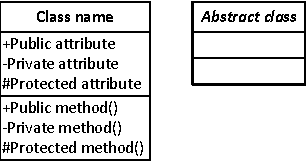
\includegraphics[width=0.35\linewidth]{img/umltheory.pdf}
\end{center}
We would like to thank our supervisor Ramin Sadre for the feedback he has given throughout the project.

\newpage
\thispagestyle{empty}
\mbox{}

\newpage
\thispagestyle{empty}
\mbox{}

\setcounter{secnumdepth}{3}
\setcounter{tocdepth}{1}

\tableofcontents*

\acresetall %resets all acronyms to not used

\linenumbers %linenumbers in the report

\chapter{Introduction}\label{chap:intro}
Many people have mobile devices, and more are getting them \todo{kilde}. Mobile devices allow for easy access to the web wherever they are, which means easier access to a vast amount of information and different kinds of media outside of your home, this includes music, video and books. The online media is becoming a good alternative to physical media because it is a lot easier to just search for it on your phone or computer. For example it is a lot easier to buy or rent an e-book than having to go to the library and borrow it. This means that in some cases books are becoming obsolete, among that are cookbooks. A physical cookbook is not going to be replaced purely by online recipes but the online recipes allow people to easily and fast search for recipes without having to borrow or buy a cookbook.

Cookbooks provide a static set of recipes, whereas a mobile device can provide you with a vast amount of recipes. Depending on the size of the device/cookbook, it might be easier to read from a mobile device and more convenient to move it around in the kitchen. A mobile cookbook can also provide a way to search for recipes and easily bookmark recipes you like.

A mobile cookbook provide the option to search for recipes when you want it. You can search for recipes while you are in the supermarket, in order to find out which ingredients you need for a specific dish. This means you do not need to plan ahead of your grocery shopping as much. Thus mobile devices allows for a way to assist you in impulse visits to the supermarket.

\chapter{Existing solutions}\label{chap:exist}
During the early stages of the project we began searching for existing solutions to draw inspiration to the design and implementation phases. All members of the group have previously had experience using different recipe sites on the Internet, and we  think that the existing solutions lack functionality. We will in this section review and discuss the existing solutions and draw some good practices from these.  

\section{Supercook}
Supercook\cite{supercook} is a website with focus on searching for recipes by their ingredients. The user is limited to enter a set of ingredients which is defined by Supercook. When adding ingredients to a search the user is aided by autocompletion and a word cloud with ingredients. The word cloud changes according to the type of ingredients you have entered, e.g. if you enter ``vanilla'' the word cloud will change to contain typical cake ingredients. It is possible to apply restrictions to your search, e.g. ``I don't eat meat''. A search on Supercook will result in a prioritised list of links to recipes from several online cookbooks. A screenshot of the website is shown in Figure \ref{fig:supercook}.

By evaluating the search results of Supercook we have deduced what we believe are the steps used to generate the search results:
\begin{enumerate}
	\item Remove recipes without matching ingredients.
	\item Sort by most matching ingredients.
	\item Sort by least missing ingredients.
\end{enumerate}
We have also noticed some quirks in the way it counts matching ingredients. It seems like the search algorithm counts the number of occurrences of the entered ingredients in the recipes. When entering ``bell pepper'' and ``olive oil'', recipes which contain both red, green, and yellow pepper are prioritised higher than recipes which actually contains both of the entered ingredients. It also appear as if ingredients in the recipes are mapped to the recipes defined by Supercook. An example of that is that ``flour'' appear to be mapped to ``flour'', ``wheat'', ``oat'', etc. This also appear to have the shortcoming that recipes containing fx ``wheat flour'' are prioritised as if they have two matching ingredient when the user entered ``flour''.

When making a search containing ``eggs'', ``garlic'', ``ground beef'', and ``onion'', we get a result which showcases a drawback of the sorting done by Supercook. The first 94 recipes are simple recipes using only few of the entered ingredients, including 24 recipes on how to boil an egg. Recipe number 95 is a recipe for meatballs and is using all entered ingredients but it also needs ``bread crumbs''. The reason why the first 94 recipes are prioritised highest is because they do not need any other ingredients than the ingredients entered.
\begin{figure}[H]
\centering
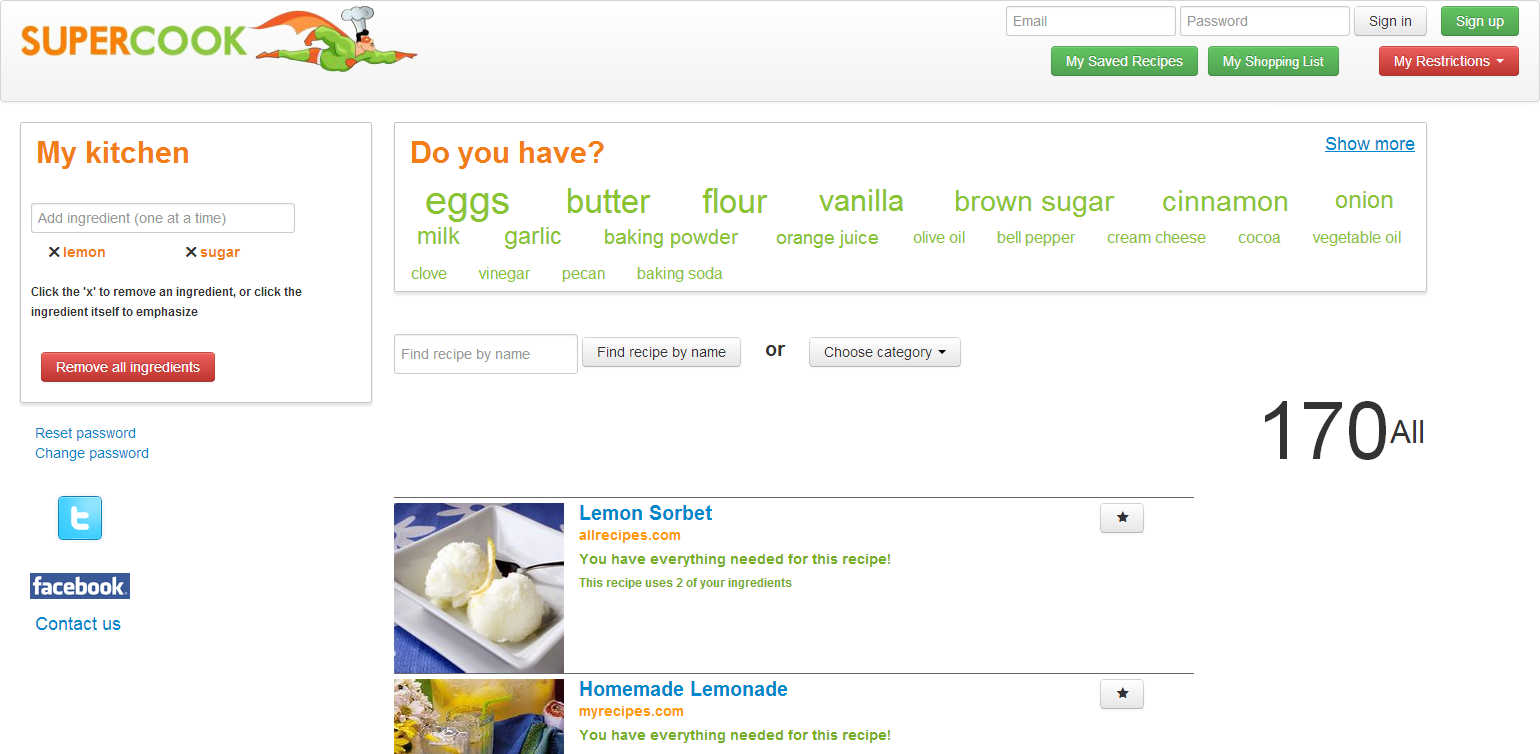
\includegraphics[width=\linewidth]{img/screenshots/supercook.png}
\caption{The inferface of Supercook.}
\label{fig:supercook}
\end{figure}

\section{Allthecooks}
Allthecooks is one of the most downloaded \cite{allthecooks-googleplay} Android applications that is related to the search: ``recipe''. The application has a great design that follows the Android guidelines\cite{guidelines-appstructure} which makes it is intuitive and easy to navigate. The detailed display of a recipe is especially well implemented, the user has everything on a single activity, and can easily see the needed ingredients and the required steps to cook the recipe. The user can also by a press of a button toggle between different measuring units, or add the selected ingredient to a shopping list. Screenshots of the application is shown in Figure \ref{fig:allthecooks-menu}, \ref{fig:allthecooks-detail1}, \ref{fig:allthecooks-detail2}, and \ref{fig:allthecooks-detail3}. The search is free-text based, which means that opposite the Supercook web application it is hard to find recipes based on ingredients. You are able to apply filters to your search to remove recipes that certain ingredients.
\twofigs{screenshots/menu.png}{Menu of Allthecooks}{fig:allthecooks-menu}{screenshots/rainbowcake-1.png}{Detail display of a recipe}{fig:allthecooks-detail1}
\twofigs{screenshots/rainbowcake-2.png}{Buttons for different features}{fig:allthecooks-detail2}{screenshots/rainbowcake-3.png}{Directions for the recipe}{fig:allthecooks-detail3}

\section{BigOven}
BigOven is also one of the most downloaded \cite{bigoven-googleplay} Android application that is related to ``recipe''. The application's navigation and design does not follow the Android guidelines\cite{guidelines-appstructure} and therefore the application's navigation can be quite confusing to an Android user. \todo{insert some pictures of the start page.} The application main page is cluttered and presents the user with many functionalities. It would be better to implement a navigation drawer and separate each function to its own view. 
It is possible to make an ingredient search and recipe search. The ingredient search is limited to only three ingredients and the algorithm finds only the recipes were they all are included, The ingredient search is based on free-text, meaning the user does not have the aid of autocompletion, like Supercook. If the user inputs three ingredients that have no real relation like; ``beef'', ``cake-mix'', ``salmon'', the ingredient search would find no results, the ingredient search excludes everything that does not contain all three ingredients. 
Like Allthecooks the user can add the different ingredients to a shopping list, save the recipe to favourites, and alternate between the metric and imperial system. 
A cool feature that is unique to the BigOven application is the Menu-Cards\todo{add picture to show how they look, they look pretty cool.} It is a small collection of different recipes that together builds to a meal, e.g. ``steak'', ``fries'', and ``green beans''. Each meal is binded to a day, which means that the user can create a Menu-Card that can contain a meal for each day of the week, or more.
The BigOven application is free, but you can buy Pro-features that exclude advertisers from the application and unlocks more functionality in the application. 

\section{Comparison}
After a small preview of the already existing solutions, of both web and android applications. We believe that we can create an application with improved features, such as a better search algorithms, easy navigation, and an elegant design. We like the idea of being able to search for recipes by ingredients, but we wont exclude the possibility to also search directly for recipes. We will also provide the user with different input styles; text-type-input(free text for recipe search and ingredient restricted), and tile-input. Tile input is basically the same as ingredient restricted input, but instead of typing the name of each ingredient the user selects the ingredient by use of tiles. The ingredient are divided into categories and maybe even subcategories, to make the navigation more sensible, otherwise the user would be presented with a too many tiles and the screen would be cluttered.

\begin{table}[H]
\centering
\begin{tabular}{|l|l|l|l|}
\hline
 & \textbf{Supercook} & \textbf{Allthecooks} & \textbf{BigOven} \\
\hline
\textbf{Platform} & Website & Android/Website & Android/Website \\
\hline
\textbf{Cost} & Free & Free & Free \& Paid \\
\hline
\textbf{Recipe search} & No & Yes & Yes  \\
\hline
\textbf{Ingredient search} & Yes & No & Yes \\
\hline
\textbf{Recipe origin} & Web crawl & User defined & User defined \\
\hline
\textbf{Shopping list} & Yes & Yes & Yes \\
\hline
\textbf{Menu planner} & No & Yes & Yes \\
\hline
\textbf{Saving recipes} & Yes & Yes & Yes \\
\hline
\textbf{Ingredient filter} & Yes & Yes & Yes \\
\hline
\textbf{Sharing of shopping list} & No & E-mail/SMS & E-mail \\
\hline
\textbf{Sharing of recipe} & No & App/SMS/E-mail & App/E-mail \\
\hline
\end{tabular}
\caption{Application comparison}
\label{tab:appcomparison}
\end{table}


\chapter{Problem definition}\label{chap:probdef}
After a small preview of the already existing solutions, of both web and android applications. We believe that we can create an application with improved features, such as a better search algorithms, easy navigation, and an elegant design. We like the idea of being able to search for recipes by ingredients, but we wont exclude the possibility to also search directly for recipes. We will also provide the user with different input styles; text-type-input(free text for recipe search and ingredient restricted), and tile-input. Tile input is basically the same as ingredient restricted input, but instead of typing the name of each ingredient the user selects the ingredient by use of tiles. The ingredient are divided into categories and maybe even subcategories, to make the navigation more sensible, otherwise the user would be presented with a too many tiles and the screen would be cluttered.




Finding recipes for cooking online has been become easy with the vast amount of sites that offer them. This has also extended to the mobile platform, allowing the users to quickly find a recipe wherever they are. It is very easy to type in the recipe you want to make and it comes up with a list of ingredients and a step by step guide on how to cook the dish.

The user does not always know exactly what dish they want to cook, but instead know which ingredients they have or what ingredients they want to use.

Being able to search for recipes based on ingredients the user already has allows them to customise their searching and receive a larger selection of dishes. It allows them to search based on items they already have in their kitchen, or based on items they know are about to go bad and they need to use. The user could also be in a situation where they see something on sale at the supermarket and quickly need to find out what dishes they can make using this ingredient.

With these problems in mind we have come up with the following problem statement for our project:

\begin{quote}
How can we take advantage of the mobile platform, in order to provide the user with relevant recipes based on specific ingredients, taking into consideration different restrictions.
\end{quote}

\chapter{Requirement}\label{chap:intro}
\section{Requirements}\label{sec:requirement}

Based on the research of existing solutions and our problem definition, we have come up with a list of requirements for our application. This list can be seen in this section.

\begin{enumerate}
  \item\label{req:android} \textbf{Android} \\
    The application must be able to run on Android version 4.3 and newer.
    
  \item\label{req:ingredientsearch} \textbf{Search by ingredients} \\
    The user must be able to search for recipes containing specific ingredients defined by the user.
    
  \item\label{req:recipesearch} \textbf{Free-text search} \\
    The user must be able to search for recipe by its title.
    
  \item\label{req:searchfilters} \textbf{Search filters} \\
    The different search methods must support filtering for users that might be allergic to certain ingredients.
    
  \item\label{req:favourite} \textbf{Favourite recipes} \\
    The user must be able to save their favourite recipes. They must also be able to remove recipes from their favourite list.
    
  \item\label{req:shoppinglist} \textbf{Shopping list} \\
    The user must be able to add and remove ingredients to a shopping list directly from the recipe. They must also be able to add and remove ingredients directly from the shopping list as well.
    
  \item\label{req:sharing} \textbf{Sharing} \\
    The user must be able to share recipes and shopping lists with other users using Facebook, Google+, E-mail, and SMS.
    
  \item\label{req:persistency} \textbf{Persistency} \\
    The system must be able to keep the user's shopping list and favourite recipes persistent.
    
  \item\label{req:unitconversion} \textbf{Unit conversion} \\
    The application must support unit conversion between the imperial system and the metric system.
    
  \item\label{req:additionallanguages} \textbf{Additional languages} \\
    The system must be ready for internationalisation.
  
  \item\label{req:Nologinrequired} \textbf{No login required} \\
    The user should not be required to log in, to use the application. Though the user might not be able to use certain features if not logged in.
\end{enumerate}

\chapter{Analysis}
\section{Story, Julie}

\newcommand{\appname}{\textbf{Flappy Cook (?)}\todo{Insert actual application name}}

Julie is in the supermarket, she does not know what to have for dinner later. She finds minced beef on sale, but she does not know what to do with it. She opens our application \appname. She is presented with an activity that says "click above to search for ingredients". She clicks the button, and then a list with categories of ingredients appears. She clicks the category called "meat", and then a word cloud appears with many different kinds of meat. In the word cloud she finds minced beef and clicks it. She now dismisses the ingredient search, and the application now presents Julie with recipes which uses minced beef. Some of the top results include Spaghetti Bolognese and Lasagne. Having not thought about this before, Julie wants to have Spaghetti Bolognese for dinner. She opens the recipe where she can see all the ingredients needed. Remembering which of the ingredients she has at home, she then adds the ingredients she needs to her shopping list. Then she favourites the recipe to easily find it later.

\section{Story, Bob}
Bob is at home, he does not know what to have for dinner later, he opens our application \appname to figure it out. Bob looks in the fridge because there might be something to use. In the fridge he finds minced meat which has a best before date set to today, so he decides that it should be used today. In the application he finds minced meat and clicks it to indicate he wants to use the ingredient. He decides he wants Spaghetti Bolognese for dinner later, but he discovers that he is missing tomato purée. He adds tomato purée to his shopping list and favourites the recipe. His wife Julie has not arrived at home yet, so instead of buying tomato purée himself, he decides to share his shopping list with Julie.

\section{Obtaining Recipes}
An application for finding recipes is not of much value without a sizeable collection of recipes. It would be a major overhead for our project if we had to create all recipes available in the system. This includes a title, description, instructions, and pictures, for each recipe.

If we want to make recipes for the system, we would undoubtedly be inspired by existing recipes. We decided to contact two lawyers to help clarify the Danish copyright law regarding recipes. Their full responses can be seen in \appref{app:copyrightmails}. It became clear that the law is quite vague about this subject. If we change some ingredients in an existing recipe we can legally call it our own.
\begin{quote}
\textit{Recipes - or culinary works if you want - are covered by copyright (in accordance with the law's § 1), as they are a kind of non-fiction works in print.}\par\raggedleft--- \textup{Erik Frodelund}, \textit{Familieadvokaten.dk}
\end{quote}
\begin{quote}

\textit{...are you using a published recipe to develop your very own recipe - for example with more ingredients and a little different quantities - you have created a new culinary work that you are free to publish in for example a book.}\par\raggedleft--- \textup{Erik Frodelund}, \textit{Familieadvokaten.dk}
\end{quote}
We are also allowed to use recipes which are considered to be ``standard-versions''. A ``standard-version'' recipe is vaguely defined as a recipe which is ``generally known''.
\begin{quote}
\textit{As long as you stick to the recipes' standard-content and approach you are not violating any rights.}\par\raggedleft--- \textup{Jørgen Lindhardt Steffesen}, \textit{Startvækst.dk}
\end{quote}
The obvious disadvantages of creating a recipe based on copyrighted material is that we need to write the description, instructions, and obtain pictures of the resulting dish ourselves.

It is also possible to obtain recipes which are licensed by a \emph{Free Cultural Works}\cite{freedomdefined} license. \emph{Free Cultural Works} are works which can be used for free, copied, and modified, for any purpose. This includes all works covered by the Creative Commons\cite{creativecommons} licenses that allow commercial use and modification of the material. The following websites contain recipes of which many are licensed by \emph{Free Cultural Works} licenses:
\begin{itemize}
	\item \url{http://en.wikibooks.org/wiki/Cookbook:Recipes}
	\item \url{http://www.nibbledish.com/}
	\item \url{http://www.opensourcefood.com/}
\end{itemize}

No matter how the recipes are obtained, we are required to adapt every recipe to fit our data structure. While some content can be crawled from the sources, different formatting between the content creators makes it hard, if not impossible, to automate the adaptation of the content to our data structure.
\section{Internationalization}
We want our system to be internationalized such that it is ready for localization.

Apart from having to provide the ability to add multiple languages, internationalization also cause other difficulties for some cultures:

\begin{description}
  \item[Reading direction] While most languages are written left-to-right top-to-bottom, some languages, like Japanese, are written top-to-bottom right-to-left.
  \item[Special characters] Some languages require characters which are not present in ASCII, e.g. ``æøå'' in Danish.
  \item[Text length] Text may be significantly longer when translated to other languages. An example is text displaying how many times an item has been viewed, e.g. ``5 views''. Translated to Italian that is written ``5 visualizzazioni''.\cite{wordlength}
  \item[Number formatting] While most of the world is using ``dot'' as the decimal mark, many cultures are using other decimal marks, like ``comma''.
  \item[Units of measure] Most of the world is using metric(SI) units for measures; however, USA, Liberia, and Burma have not yet adopted the metric system.\cite{unitsfactbook}
  \item[Prohibited foods] Some types of food may be prohibited or tabooed in certain cultures and religions.
\end{description}

\chapter{Design}\label{chap:design}
\section{Prototypes}
This section shows the prototypes that we have made and touches lightly on the application's functionality. The section includes both early and late prototypes to show how the design has progressed and changed. \todo{Billede af start screen}

\begin{figure}[H]
\begin{minipage}[b]{0.5\columnwidth}
\centering
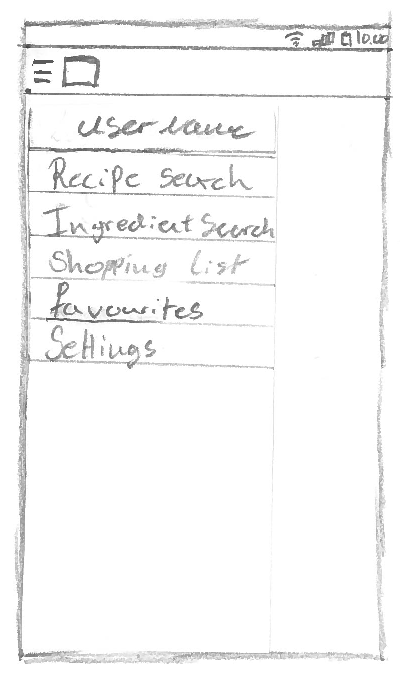
\includegraphics[width=0.7\columnwidth]{img/prototypes/navigation_drawer.pdf}
\caption{The navigation drawer\label{fig:navdrawer}}
\end{minipage}
\hspace{0.5cm}
\begin{minipage}[b]{0.5\columnwidth}
\centering
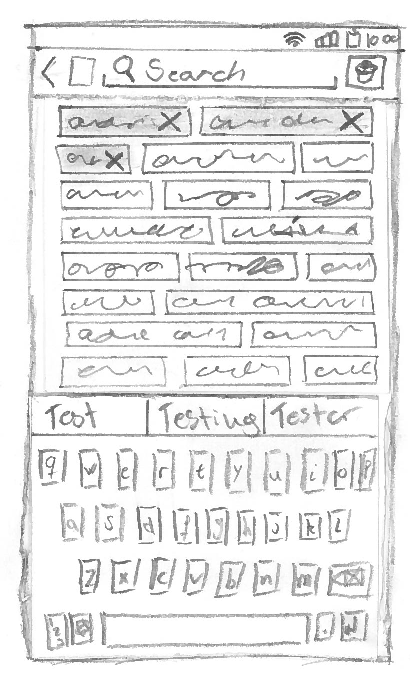
\includegraphics[width=0.7\columnwidth]{img/prototypes/ingredient_search_text.pdf}
\caption{Ingredient search with text\label{fig:ingretext}}
\end{minipage}
\end{figure}

The first thing the user is shown when opening the application is the navigation drawer, as seen on \autoref{fig:navdrawer}. This is a standard component in Android which is used to navigate between different pages. We chose to use this design because we want to follow the guidelines provided by Google\cite{guidelines-appstructure}, and we felt it was a good way to make the views less cluttered, collecting all navigation options in an easy accessible component.

The application allows the user to search for recipes both based on the title of the recipe and based on ingredients that the user inputs. Searching for recipes based on the title is simple and straight forward, the user inputs a partial or full title of the recipe they want and the application shows suggestions based on this. Searching based on ingredients is more complicated. The user might have to type in multiple ingredients and we want to make it easy for them to do so, therefore we have implemented two different ways of aiding the user in entering ingredients, either by text or by tiles.

\autoref{fig:ingretext} shows the screen layout when entering ingredients with text. The user clicks the search field at the top of the page and a keyboard and a word cloud pops up. Now the user can either type in the ingredient they want by use of the keyboard, or if the word appears in the word cloud they can simply click it. The idea with the word cloud is that it comes up with suggestions based on the ingredients the user has already put in.

\begin{figure}[H]
\begin{minipage}[b]{0.5\columnwidth}
\centering
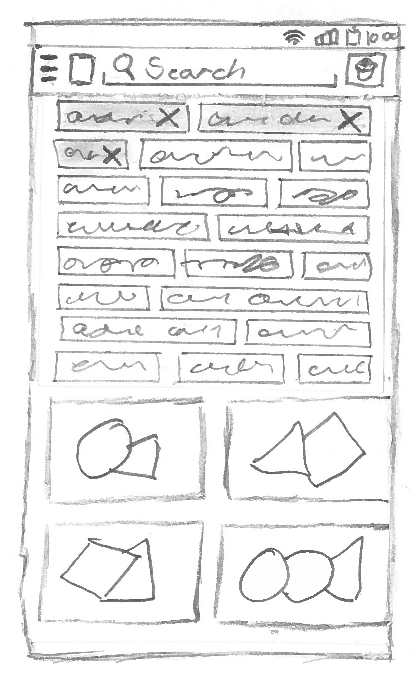
\includegraphics[width=0.7\columnwidth]{img/prototypes/ingredient_search_tile.pdf}
\caption{Ingredient search with tile selection\label{fig:ingreani}}
\end{minipage}
\hspace{0.5cm}
\begin{minipage}[b]{0.5\columnwidth}
\centering
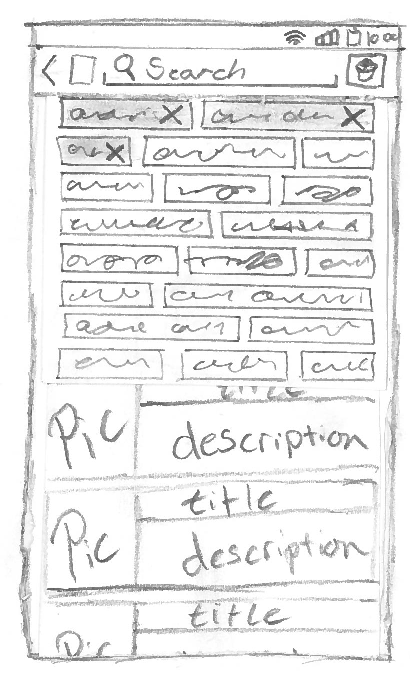
\includegraphics[width=0.72\columnwidth]{img/prototypes/recipe_browse.pdf}
\caption{Recipe browsing with a word cloud\label{fig:recipecloud}}
\end{minipage}
\end{figure}

The same idea applies when entering ingredients using tiles, but instead of a keyboard a small tile bar pops up. This bar contains the different categories, and the user can click on one of these in order to go deeper down into a category, as the user navigates deeper the word cloud will update with words associated with the category they are browsing. The tile navigation can be seen on \autoref{fig:ingreani}. When the user is done with inputting their ingredients they press the back button to close the keyboard or the tiles and can browse the suggested recipes. \autoref{fig:recipecloud}, \autoref{fig:recipestatic}, and \autoref{fig:recipenothing} are three different versions of what it will look like when the user does so.

\autoref{fig:recipecloud} shows the same page without the keyboard, giving the user access to browse the suggested recipes while still having access to the word cloud allowing them to remove or add new ingredients on the fly, however the drawback is a very small view of the suggested recipes. 

\begin{figure}[H]
\begin{minipage}[b]{0.5\columnwidth}
\centering
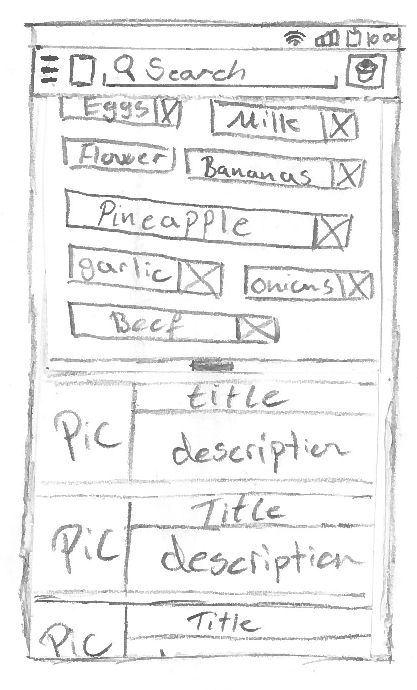
\includegraphics[width=0.7\columnwidth]{img/prototypes/recipe_browse2.pdf}
\caption{Recipe browse with static ingredients\label{fig:recipestatic}}
\end{minipage}
\hspace{0.5cm}
\begin{minipage}[b]{0.5\columnwidth}
\centering
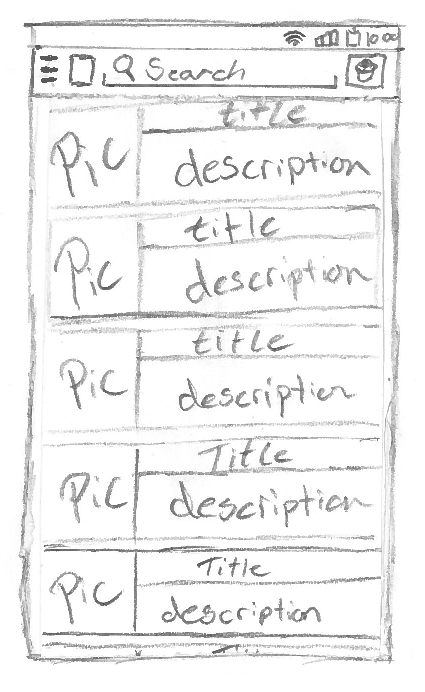
\includegraphics[width=0.7\columnwidth]{img/prototypes/recipe_browse3.pdf}
\caption{Recipe browse without ingredients\label{fig:recipenothing}}
\end{minipage}
\end{figure}

\autoref{fig:recipestatic} shows the page without the keyboard or word cloud but only the selected ingredients, allowing the user to remove items on the fly, again the drawback is a rather small view for the suggested recipes.

\autoref{fig:recipenothing} only shows the suggested recipes, allowing the user to see more recipes but having to click the search field again in order to edit their ingredients.

\begin{figure}[H]
\begin{minipage}[b]{0.5\columnwidth}
\centering
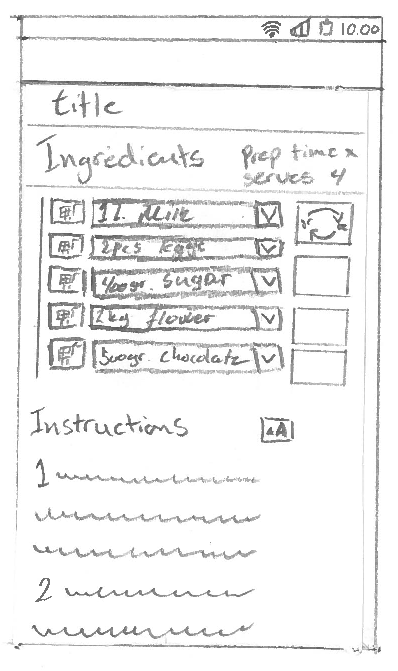
\includegraphics[width=0.7\columnwidth]{img/prototypes/recipe_old.pdf}
\caption{First layout for the recipe view\label{fig:recipeold}}
\end{minipage}
\hspace{0.5cm}
\begin{minipage}[b]{0.5\columnwidth}
\centering
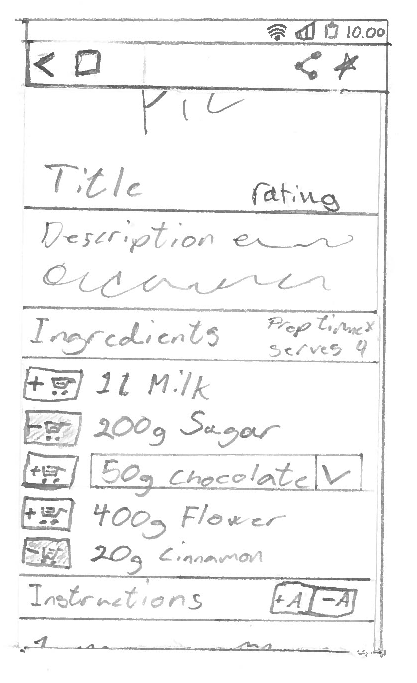
\includegraphics[width=0.735\columnwidth]{img/prototypes/recipe_new.pdf}
\caption{Redesigned recipe layout\label{fig:recipenew}}
\end{minipage}
\end{figure}

When the user finds a suggested recipe they want to look at, they press it and they are taken to a new page. The two variants of this page is shown on \autoref{fig:recipeold} and \autoref{fig:recipenew}. The three vertical lines in the top left corner have been replaced with a back arrow, this indicates two things; the navigation drawer is not available on this page and the back arrow indicates that if you click it you will be taken back to the previous page which is the list of suggested recipes.

In the top right corner there are two new icons; the first button is the share button, allowing the user to share the recipe with their friends and family. The second button is the favourite button, the user can click this to save the recipe under their favourites if they click it again they unfavourite it.

\autoref{fig:recipeold} shows the first design, under the action bar there is a picture of the dish and just under that the title. This is followed by a list of ingredients and the instructions for making the dish. Next to "Ingredients" the user can see the time it takes to prepare the dish, and how many people the dish will serve.

To the left each ingredient there is a button with a shopping cart icon, the user can press this in order to add this ingredient to their shopping list. If the user presses the same icon again, the ingredient is removed from the shopping list. By default the application assumes that the user does not have any of the ingredients, so the user has to choose which ingredients they need to add to the shopping list.

Each of the ingredients have a box around them and a down arrow, this is to indicate a drop down menu. These will appear when an ingredient is exchangeable according to the recipe, meaning the user can use something else similar and still use the recipe. To the right of the ingredients there is a button with a circle on it. If the user presses this button all the unit measures in the recipe will be converted between Imperial and Metric and visa versa. Under the list of ingredients there is a list of instructions telling the user how to cook the dish. The button labelled "aA" next to instructions can be pressed and different font sizes can be chosen.

To the right of the ingredients there is a button with a circle on it. If the user presses this button all the unit measures in the recipe will be converted between Imperial and Metric and visa versa. Under the list of ingredients there is a list of instructions telling the user how to cook the dish. The button labelled "aA" next to instructions can be pressed and different font sizes can be chosen.

We redesigned this layout and the result can be seen on \autoref{fig:recipenew}. Most of the changes are small changes to previous design, for example the location of the title. It has now been moved up onto the picture, together with a rating for the recipe. There is now a small description under the recipe describing the dish. The shopping carts now have a small "+" or a small "-" to indicate if the user will add or delete the ingredient when they press it. We kept the drop down menu for ingredients to indicate that an ingredient is exchangeable. Instead of the "aA" icon that the user should press, there are now two buttons, one to make the font larger and one to make it smaller.

One of the larger redesigns we did, was that we removed the buttons to the right of the ingredients as we decided to add their functionality elsewhere and therefore have more room for the ingredient names.

\begin{figure}[H]
\begin{minipage}[b]{0.5\columnwidth}
\centering
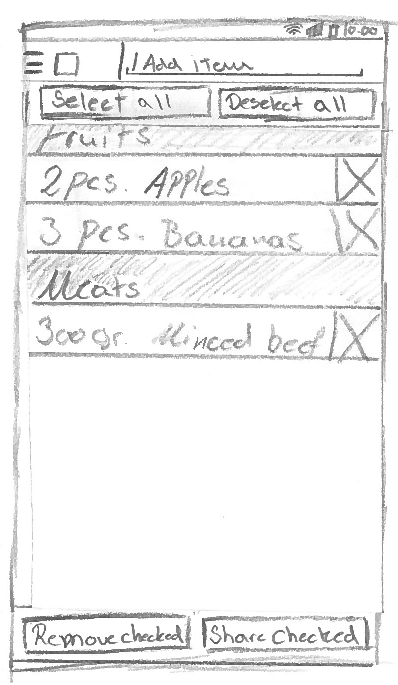
\includegraphics[width=0.7\columnwidth]{img/prototypes/shopping_list_old.pdf}
\caption{First layout for the shopping list\label{fig:shoppingold}}
\end{minipage}
\hspace{0.5cm}
\begin{minipage}[b]{0.5\columnwidth}
\centering
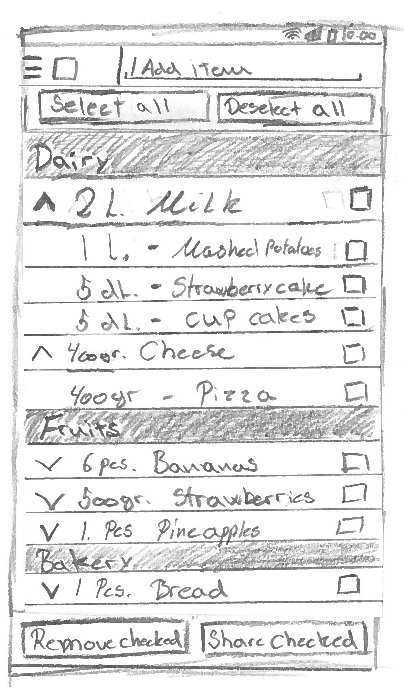
\includegraphics[width=0.7\columnwidth]{img/prototypes/shopping_list_new.pdf}
\caption{Redesigned layout for shopping list\label{fig:shoppingnew}}
\end{minipage}
\end{figure}

The user can always access their shopping list through the navigation drawer. \autoref{fig:shoppingold} and \autoref{fig:shoppingnew} shows the early design and redesign of the shopping list. The user is able to add ingredients directly in the shopping list by clicking the "Add item" field at the top. They are also able to quickly select or deselect all items in the list by clicking the "Select all" or "Deselect all" button under the action bar. This is useful if the user wants to remove all the ingredients or share them all. This can be done through the two buttons at the bottom of the page.

\autoref{fig:shoppingold} shows the first design of the shopping list, it displays how much of each ingredient the user needs, it has a simple layout where ingredients are divided into categories so the user has an easy overview of it. \autoref{fig:shoppingnew} shows a redesigned version of the shopping list. The design takes what recipes the ingredients come from into consideration. This means that if the user needs 2L of milk, they can click on it and see in which recipes they need how much milk. It also makes it easier for the user to remove ingredients if they decide not to make a specific recipe.

\begin{figure}[H]
\begin{minipage}[b]{0.5\columnwidth}
\centering
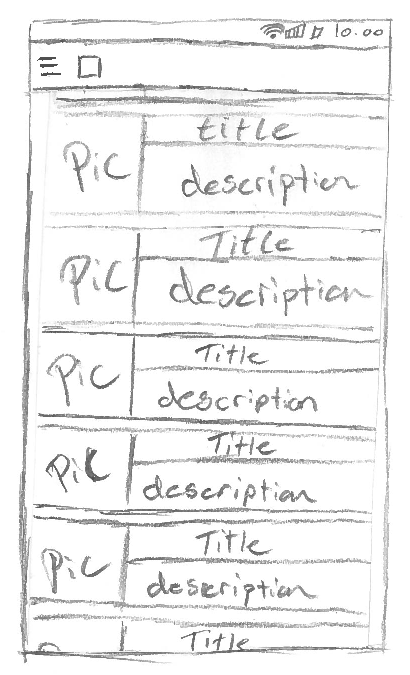
\includegraphics[width=0.7\columnwidth]{img/prototypes/favorites.pdf}
\caption{The layout for favourites\label{fig:favourite}}
\end{minipage}
\end{figure}

As mentioned before the user can favourite a recipe by clicking the icon when looking at a recipe. \autoref{fig:favourite} shows the favourite page, it looks a lot like \autoref{fig:recipenothing} but it does not have the share or favourite button at the top. The user unfavourites a recipe either by long clicking the recipe or click it to go into the recipe and click the star symbol to unfavourite it.



\bookmarksetup{startatroot}% dette skulle stoppe part, så conclusion får indryk. Problemet i skrivende øjeblik er at chapters har samme indryk uafhængigt af parts
\addtocontents{toc}{\bigskip}%laver ekstra mellemrum

\chapter{Conclusion}
The focus of this project was to make an application that would take advantage of the mobile platform and provide the users with relevant recipes based on specific ingredients. Furthermore we wanted to support any user defined restrictions, like allergies.
This is defined in our problem definition from \chapref{chap:intro}:
\begin{quote}
How can we take advantage of the mobile platform, in order to provide the user with relevant recipes based on specific ingredients, and taking any user defined restrictions, like allergies, into consideration.
\end{quote}
In order to make the application easy for the users to use, a problem that had to be solved was how the users should navigate the application. We decided to use the navigation drawer and display it the first time the application is opened. We chose the navigation drawer because it is recommended to use when the application has more than three top level views in order to give the user an overview of the application.

The application itself consists of three pages, a page to search by ingredient, a page to search for recipes using free-text, and a favourite page. 

When the user wants to search for recipes using ingredients, they click the search field, ingredients and a word cloud appear filled with already predefined ingredient suggestions. The user is able to click these and add them to the search, they are also able to search for ingredients using text. When the user types in the search field they are given a list of suggestions based on the letters they have already typed. The user can either click an ingredient in the list to add it to the search or click the enter button on the keyboard to add the first suggestion in the list to the search. When the user is done entering ingredients they can perform a search by clicking the enter button while having an empty search field. This closes the word cloud and searches for recipes based on the ingredients that were selected. 

The user is given a list of recipes that either include all or some of the ingredients that they entered. The recipes are prioritised accordingly to our precedence function described in \secref{sec:design_search}. The user can click a recipe from the list to open a page showing the full recipe. The users are able to favourite recipes by clicking the star in the top right corner. In order to favourite recipes they must be signed in through Google+. As long as they are signed in the users can always access the recipes through the favourite page. Through the favourite list they can also remove favourites by long clicking and click "remove" when prompted. They can also remove a favourite recipe by clicking the star in a favourited recipe.

The user is also able to search for recipes using free-text using wildcards such as *, + and "". In order to receive a result from the free-text search, the input text has to match either parts of the recipe name or part of the description of a recipe. A match on the recipe title is prioritised over a match on the description, and a match on both title and description is prioritised over a match on the title.

Due to time constraints, we have not managed to fulfil all of our initial requirements as listed in \secref{sec:requirement}. One of the major features that is lacking is the shopping list. It proved more complicated and time consuming to implement than first anticipated due to too much UI design on the application.

The intended purpose of the word cloud was to provide the user with relevant suggestions based on the ingredients they already entered to the search, however at the moment the suggestions provided are static and does not change. This basic implementation was a result of time constraints and how complicated it proved to implement something that gives relevant results. 

As the project progressed, we chose to focus on developing a working application with a few core features which meant that features such as search filters, sharing, persistency, unit conversion, and additional languages where deprioritised. 

Based on the tests performed in \chapref{chap:tests}, we can guarantee\todo{nej} that the server returns a correct and valid \ac{json} format to the mobile application. Our black box test shows that the mobile application's functionalities works. We have not made any graphical user interface tests to ensure the design of our mobile application and website. We have managed to create an application which provides the users with the ability to search for recipes based on ingredients or using free-text.\label{chap:conclusion}

%\chapter{Future Work}
%Due to time constraints in our project we have not managed to implement all functionalities. This chapter describes the features we did not have time to implement, but would like to implement in the future.

\begin{description}
\item[Shopping list] We wanted to have a shopping list where ingredients could easily be added from recipes and also from the shopping list itself.

\item[Start page] The application needs some kind of a start page, right now the application opens in the ingredient search page. The start page can be a page displaying popular or featured recipes to inspire the user, but an automatic display of popular recipes might become a static page with the same recipes displayed, and featured recipes needs to be maintained. Another option for a start page can be a welcome message and a small guide or tutorial on how the application works and what it does.

\item[Recipe filters] The user should be able to specify some filters for search results. Examples are filters for vegans and allergies.

\item[Sharing] You cannot currently share anything in the application. We wanted the ability to share recipes and shopping lists. Sharing can happen through services like SMS, Facebook, or Google+.

\item[Recipe cache] Right now the recipes are downloaded each time they are opened. All the images are already automatically cached in the application, caching recipes also makes sense, since they are probably likely to opened multiple times, especially when they are favourited for later use.

\item[Recipe license] We need to display a license on all the recipes in the application, the application can currently display a license, but the server does not send it.

\item[Conversion] The database and the model currently contains a conversion constant for each unit, but the application does not contain the functionality to convert between units. Right now in the database decilitre is converted to ounces, but usually the imperial system deals with cups.

\item[Recipe references] We wanted recipes to be able to have references to other recipes, because ingredient groups might be big enough to be its own recipe. This is currently not possible.

\item[Settings] The application does not have a settings page. Settings could include: Metric or imperial standard option, filtering of recipes, and language.

\item[Scaling of recipes] Button to scale the ingredients of a recipe to more people.

\item [Intelligent sort of ingredients] Instead of having a static word cloud like we have now, we want the word cloud to update each time a user adds an ingredient to their search. We want the word cloud to update with suggestions based on the ingredients already added.

\item [User created recipes] In order to increase the collection of recipes, the users should be able submit their own recipes.

%\item Shoppinglist
%\item Settings
%\item Salt er der som ingrediens? Settings?
%\item Startpage
%\item Conversion
%\item Filter (vegan)
%\item Refs to other recipes
\item [Localisation] At the moment the application only supports English. We want to support more languages in the future in order to reach a wider audience.
%\item Share recipes and shopping lists (sms, facebook, google+)
\item [Log interesting ingredient searches] It could be very interesting to log what ingredients the users searches for the most. This could identify which ingredients the user search for and maybe help us improve our selection of recipes. It might help to improve the word cloud by identifying what ingredient combinations are mostly used.
%\item Recipe cache on mobile device (Perhaps FIFO)
%\item llicense på recipes
\item [Revoke Google account access]
The user should also have the option to revoke access, meaning the application would reset the granted access to the user's Google+ account.
This option should be implemented in the settings menu.
\end{description}


\begin{appendices}
\chapter{First Appendix}\label{appendixStart}
% next appendix
\label{appendixEnd}
\end{appendices}

\cleardoublepage
\listoffigures*

%\cleardoublepage
%\listoftables*

\cleardoublepage
\renewcommand{\lstlistlistingname}{List of Listings}%ændrer overskriften
\lstlistoflistings

% Afslut med bibliografien. Bibliografien har mærkelige sidetal og side reference. Fixed med cleardoublepage og phantomsection
\cleardoublepage
\phantomsection
\label{chap:bib}% brugt i preface
\bibliography{bib/bibliografi}

\label{lastpage}% brugt i titelblad til total sidetal

% hvis den sidste side er et lige sidetal så skal der indsættes en ekstra blank bagside
\ifthenelse{\isodd{\pageref{lastpage}}}
{% ulige sidetal = højre side
% do nothing
}
{% lige sidetal = venstre side
\pagebreak
\thispagestyle{empty}
\mbox{}
}

\end{document}
